\section{Conceptual Designs}

As many design decisions depend on the airframe of the system, a process of ideation and concept generation was identified as a priority for the project. The following section outlines the approach taken to ensure innovation was facilitated while adhearing to the timeline.

\subsection{Concept Generation Approach}
\label{sec:Concept_Generation_Approach}

% What are we doing
% Approach to what
% How does this impact the project
% Why is it important
% What order were things conducted
% what were the outcomes

To effectively develop concepts that would have potential to push the flight efficiency technology curve, existing literature and aircraft designs were studied. Based on this research, design gaps pertaining to efficient VTOL aircraft design were identified and explored. With the existing technology in mind, a first principles approach to airframe design was conducted. This method allowed the team to eliminate any assumptions and propositions that had the potential to constrain the creativity of the concept generation.

\subsubsection{Methodology}

A set of specific, relevant, measurable and scalable performance criteria were derived from the primary objectives to ensure the concepts aligned with the project requirements. These criteria are detailed in Section \ref{perfcrit}.\\

The first round of concepts were assessed against the performance criteria, using theoretical analysis based on literature and qualitative reasoning. The concepts were then ranked based on their score for each objective, and the top scoring concepts were analysed. This process allowed the team to rapidly identify the most relevant and successful technologies when considering the specific domains defined by the project objectives. This information allowed the team to focus the concept generation ideation for the second iteration embed synergies within the design.\\

This approach is summarised below.
\begin{enumerate}
    \item Review the existing literature and designs in the aircraft design field.
    \item Identify the main characteristics of existing designs.
    \item Generate performance criteria from project objectives.
    \item Creatively theorise potential concepts using first principles.
    \item Rank concepts based on performance criteria.
    \item Further iterate top ranked concepts and generate additional concepts by designing for objectives.
    \item Assess modified/new concepts against the performance criteria and further develop the top ranked concepts.
\end{enumerate}

\subsubsection{Desired Outcomes}

This approach is designed to eliminate concepts that do not align with the project aim and converge on a concept that broadly does. To ensure scope for innovation was maintained, a wide variety of concepts were developed. The desired outcome of this process was to give the team a broad understanding of the advantages and disadvantages associated with particular designs and to decide on an airframe concept that could then be further developed and refined. The decided concept would then be used as base design upon which tests could be conducted and improvements could be made. As the concept was not intended to be the final product, the process was not designed find the optimal system, but instead act as a method to decide on a system worthy of further investigation.


% \begin{itemize}
%     \item Find a design that's suitable
%     \item Not necessarily finding an optimal design
%     \item Not a critical evaluation of concepts
%     \item Only aimed at deciding on a design for further analysis
% \end{itemize}

\subsubsection{Limitations}

Given the number of concepts developed and the constrained timeframe, it was deemed appropriate to take a somewhat qualitative approach to scoring the concepts against some of the performance criteria. With more time and resources, prototyping could be conducted to achieve definitive results upon which to base the concept assessments.

\subsection{Performance Criteria}\label{perfcrit}


Table \ref{tab:objectives} attributes each objective with its respective numerical identifier used throughout this section.

\begin{table}[H]
\caption{Project Objectives}
\label{tab:objectives}
\centering
\begin{tabular}{|c|p{10cm}|}
\hline
             \#                       & \multicolumn{1}{c|}{\textbf{Description}} \\\hline
1 & Design and Manufacture an Airframe                                    \\
2 & Design Complies with Standards and Regulations                                     \\
3 & Design System Capable of Forward Flight                                                \\
4 & Design System Capable of Hovering                                                \\
5 & Design System with Payload Capacity                                                                   \\
6 & Design System to Perform VTOL Transitions                                                               \\
7 & Design System to Perform Autonomous Operations                                                              \\\hline
\end{tabular}
\end{table}



\subsubsection{Assessed Attributes for Objectives}
%explain selection criteria
%include large selection criteria table

% Tod do: discuss and justify criteria within each objective.\\
In order to achieve the project aims, each objective was broken down into its key capabilities and characteristics that would be required to achieve it. These are summarised in Table \ref{tab:objective-attributes-weightings} and further detailed in Appendix \ref{app_performance_criteria}.

% Tables \ref{tab:obj_1_criteria} to \ref{tab:obj_6_criteria} in Appendix  show the performance criteria that were developed to compare airframe designs. 









% \newgeometry{left=1.5cm, right=0.5cm, bottom=0.5cm, top=0.5cm}
% % \begin{landscape}
% \pagestyle{empty}




% \end{landscape}
% \restoregeometry
% \clearpage

\subsubsection{Weightings}

Table \ref{tab:objective-attributes-weightings} also shows the relative weightings applied to each objective when considering their respective performance criteria. Note that Objective 2 and 7 are not included in the weighting because they are considered independent of the airframe design.

\begin{table}[H]
\caption{Objective Attributes and Weightings}
\label{tab:objective-attributes-weightings}
\centering
\begin{tabular}{|c|p{10cm}|r|}
\hline
\multicolumn{1}{|c|}{\textbf{Obj. \#}}     & \textbf{Sample Attributes}           & \multicolumn{1}{c|}{\textbf{Weighting}} \\\hline
1 & Manufacturing simplicity, durability, reliability, weight, cost                                     & 0.14                                   \\\hline
2 &  Weight category, autonomy requirement, certified pilot availability & -                                      \\\hline
3 &  Forward aerodynamic efficiency, propulsive efficiency, endurance, controllability & 0.24                                   \\\hline
4 &  Vertical aerodynamic efficiency, propulsive efficiency, endurance, controllability                                      & 0.24                                   \\\hline
5 &  Size and weight range accepted, ease of insertion, impact on flight                                  & 0.16                                   \\\hline
6 &  Transition time and efficiency, transition requirements, robustness,                               & 0.22                                   \\\hline
7 &  Reliability, degree of automation, conditions required                         & -                                      \\\hline
 \multicolumn{1}{|c}{}   &        \multicolumn{1}{r|}{Total}                       & 1.00                                     \\\hline
\end{tabular}
\end{table}

Objectives 3 and 4 have the highest weighting as they pertain to the efficiency of the airframe and are therefore crucial to the overarching aim of pushing the range capabilities of the system. Objective 6 refers to the VTOL transition efficiency and is therefore considered of similar importance for the same reasons. Objectives 5 is weighted less as the payload requirements for the CFS are fairly limited. Objective 1 is weighted the least as most concepts will be able to be manufactured by either the Mechanical Engineering Workshop or by external manufacturers.\\

Within each objective, the various criteria are weighted to allow for consideration for the differing level of importance. These criteria and their respective weights can be seen in the tables within Appendix \ref{app_performance_criteria}.


\subsection{Airframe Concepts}

As stated in Section \ref{sec:Concept_Generation_Approach}, an iterative approach was used to generate and improve upon airframe concepts. The following sections detail a selection (not all) of concepts from each round of analysis. 

\subsubsection{Round 1 Concepts}
% Show the basic images of the desings
%include description and advantages/disadvantages in appendix (similar to ATLAS report) 
% Include the performance score and the visual displaying strengths and weaknesses
% * This section will show CAD drawings and radar charts of selected concepts. An example of the layout (minus a CAD drawing) is given below.\\
% \note{Rhys}{1-[Rhys],5-[Jake],6-[Peter],12-[Sam],8-[Harry]}\\
% \note{Rhys}{Actually show/visualise score for each desing}\\
% \note{Rhys}{Make a note why objective 2 and 7 arnt in this analysis}\\
% \note{Rhys}{Round 1=6 designs. Round 2=4 designs. Round 3=2 designs}\\

The Round 1 concepts draw on inspiration from literature and a first principles analysis of aerofoils. The scores from this round were used as a benchmark for further concepts. 

\paragraph{Concept 1: Commercially Available VTOL UAV}
This fixed wing fuselage UAV features a channelled wing design to promote more lift at low speeds and therefore reduce stall speeds. The four motors for hover and VTOL capabilities allow for high stability as they are placed away from the centre line and therefore produce a larger moment to counter disturbances. One horizontal pusher motor is used in forward flight, simplifying transition as no motor rotation is required. This leads to inefficiencies however as during both flight modes there are motors that are not active and are essentially dead weight. Due to the channelled wing, manufacturing complexity is increased. Figure \ref{fig:concept1} shows the concept and its performance criteria assessment results. 



\begin{figure}[H]
\centering
\begin{subfigure}[t]{.5\textwidth}
  \centering
  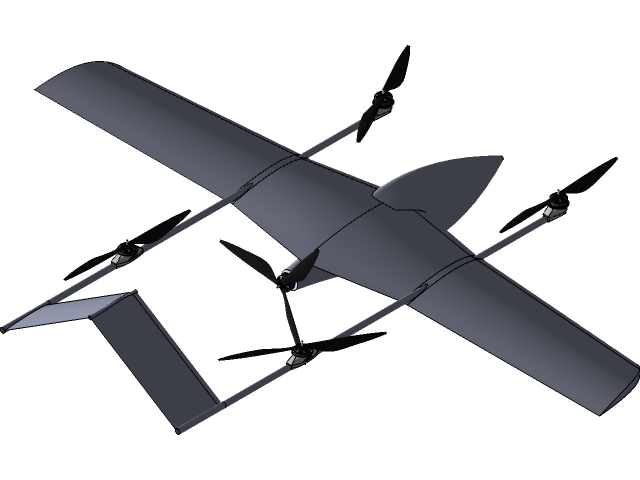
\includegraphics[width=0.85\linewidth]{Concepts/CAD/1cad.png}
  \vspace{0.125cm}
  \caption{CAD Drawing}
  \label{fig:cad1}
\end{subfigure}%
\begin{subfigure}[t]{.5\textwidth}
  \centering
  \fbox{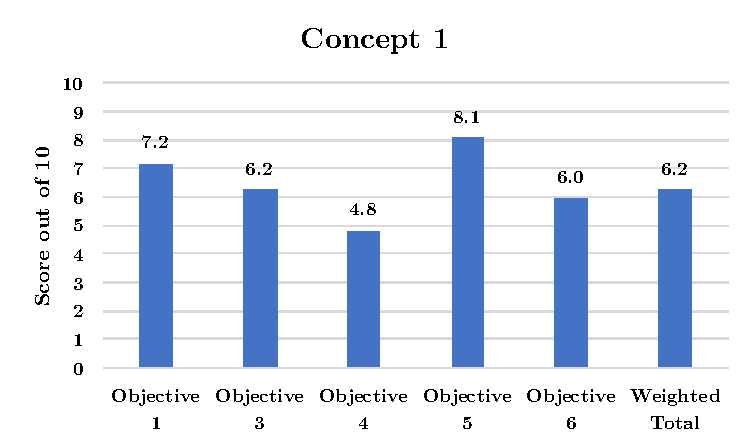
\includegraphics[width=0.95\linewidth]{Concepts/Plots/1.pdf}}
  \caption{Performance Criteria Assessment Results}
  \label{fig:radar1}
\end{subfigure}
\caption{Concept 1 - Commercially Available VTOL UAV}
\label{fig:concept1}
\end{figure}


\paragraph{Concept 2: Single Puller Propeller Tailsitter}
This tailsitter uses a large diameter propeller for propulsion and two smaller propellers mounted perpendicularly for stabilisation. The large diameter of the main propeller increases efficiency in both hover and forward flight modes, but the large wetted area causes significant amounts of drag at high speeds. The system does not require any moving parts other than the motors, therefore reducing manufacturing complexity. Due to the nature of tailsitters, the payload is not oriented in the same plane during all flight modes. This design therefore requires additional systems such as gimbals or extra sensors to maintain a consistent relevant data feed from the payload. Figure \ref{fig:concept2} shows this design and its performance.



\begin{figure}[H]
\centering
\begin{subfigure}[t]{.5\textwidth}
  \centering
  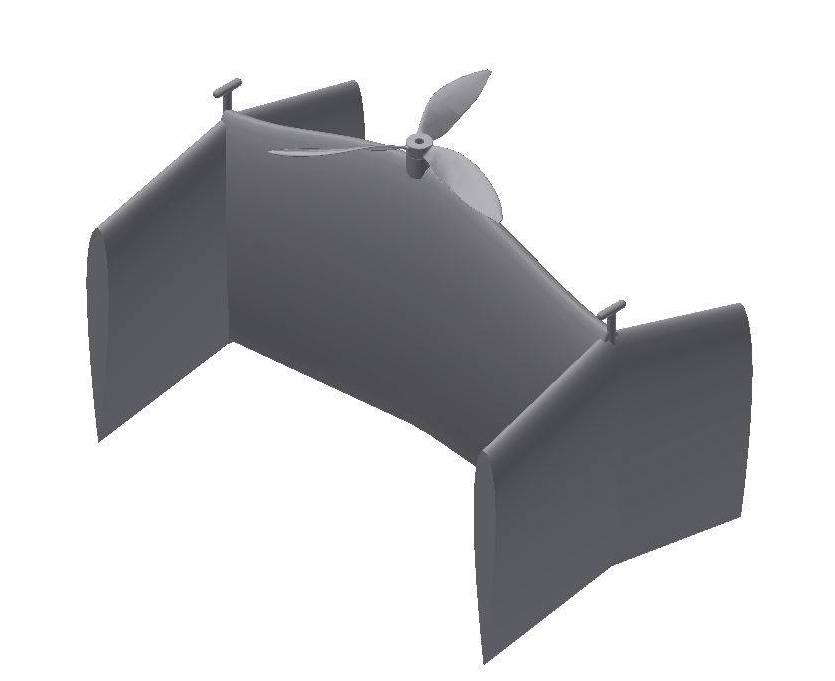
\includegraphics[width=0.75\linewidth]{Concepts/CAD/5cad.jpg}
  \vspace{0.125cm}
  \caption{CAD Drawing}
  \label{fig:cad2}
\end{subfigure}%
\begin{subfigure}[t]{.5\textwidth}
  \centering
  \fbox{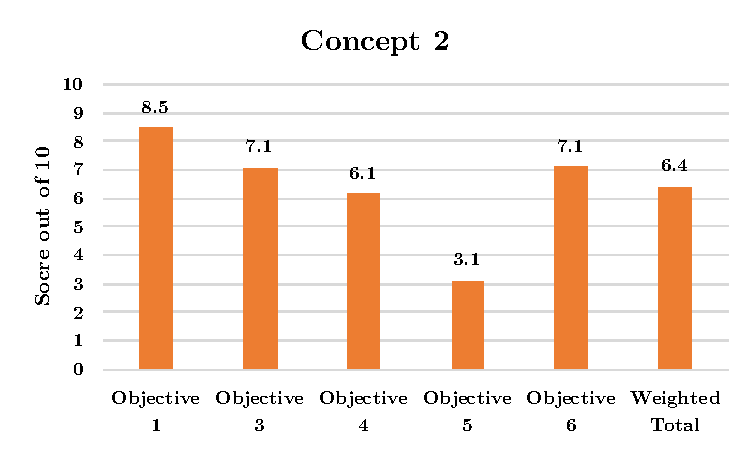
\includegraphics[width=0.95\linewidth]{Concepts/Plots/5.pdf}}
  \caption{Performance Criteria Assessment Results}
  \label{fig:radar2}
\end{subfigure}
\caption{Concept 2 - Single Puller Propeller Tailsitter}
\label{fig:concept2}
\end{figure}


\paragraph{Concept 3: Distributed Lift Tilt Wing}
This concept leverages the increased efficiency from distributed propulsion over the main wing in both forward flight and hover modes by incorporating a wing tilting mechanism. Efficiency will can be further increased by overlapping the propellers and adding the ability to deactivate motors to reduce power consumption if required. A tilt tail pusher is included to add stability in hover modes while also adding thrust during forward flight. Figure \ref{fig:concept3} shows this design and its performance.

% Tilt-wing, distributed lift design with a tilt tail pusher. Wing is integrated into main fuselage, housing tilting mechanism. Pusher tilt mechanism is housed in the rear of the fuselage.  Main lift system is the distributed lift over the wing, using smaller but more efficient motors and by overlapping disk areas of props will increase efficiency of lift generation. Can possibly include a system to deactive certain motors on the wing to save power if required. 

\begin{figure}[H]
\centering
\begin{subfigure}[t]{.5\textwidth}
  \centering
  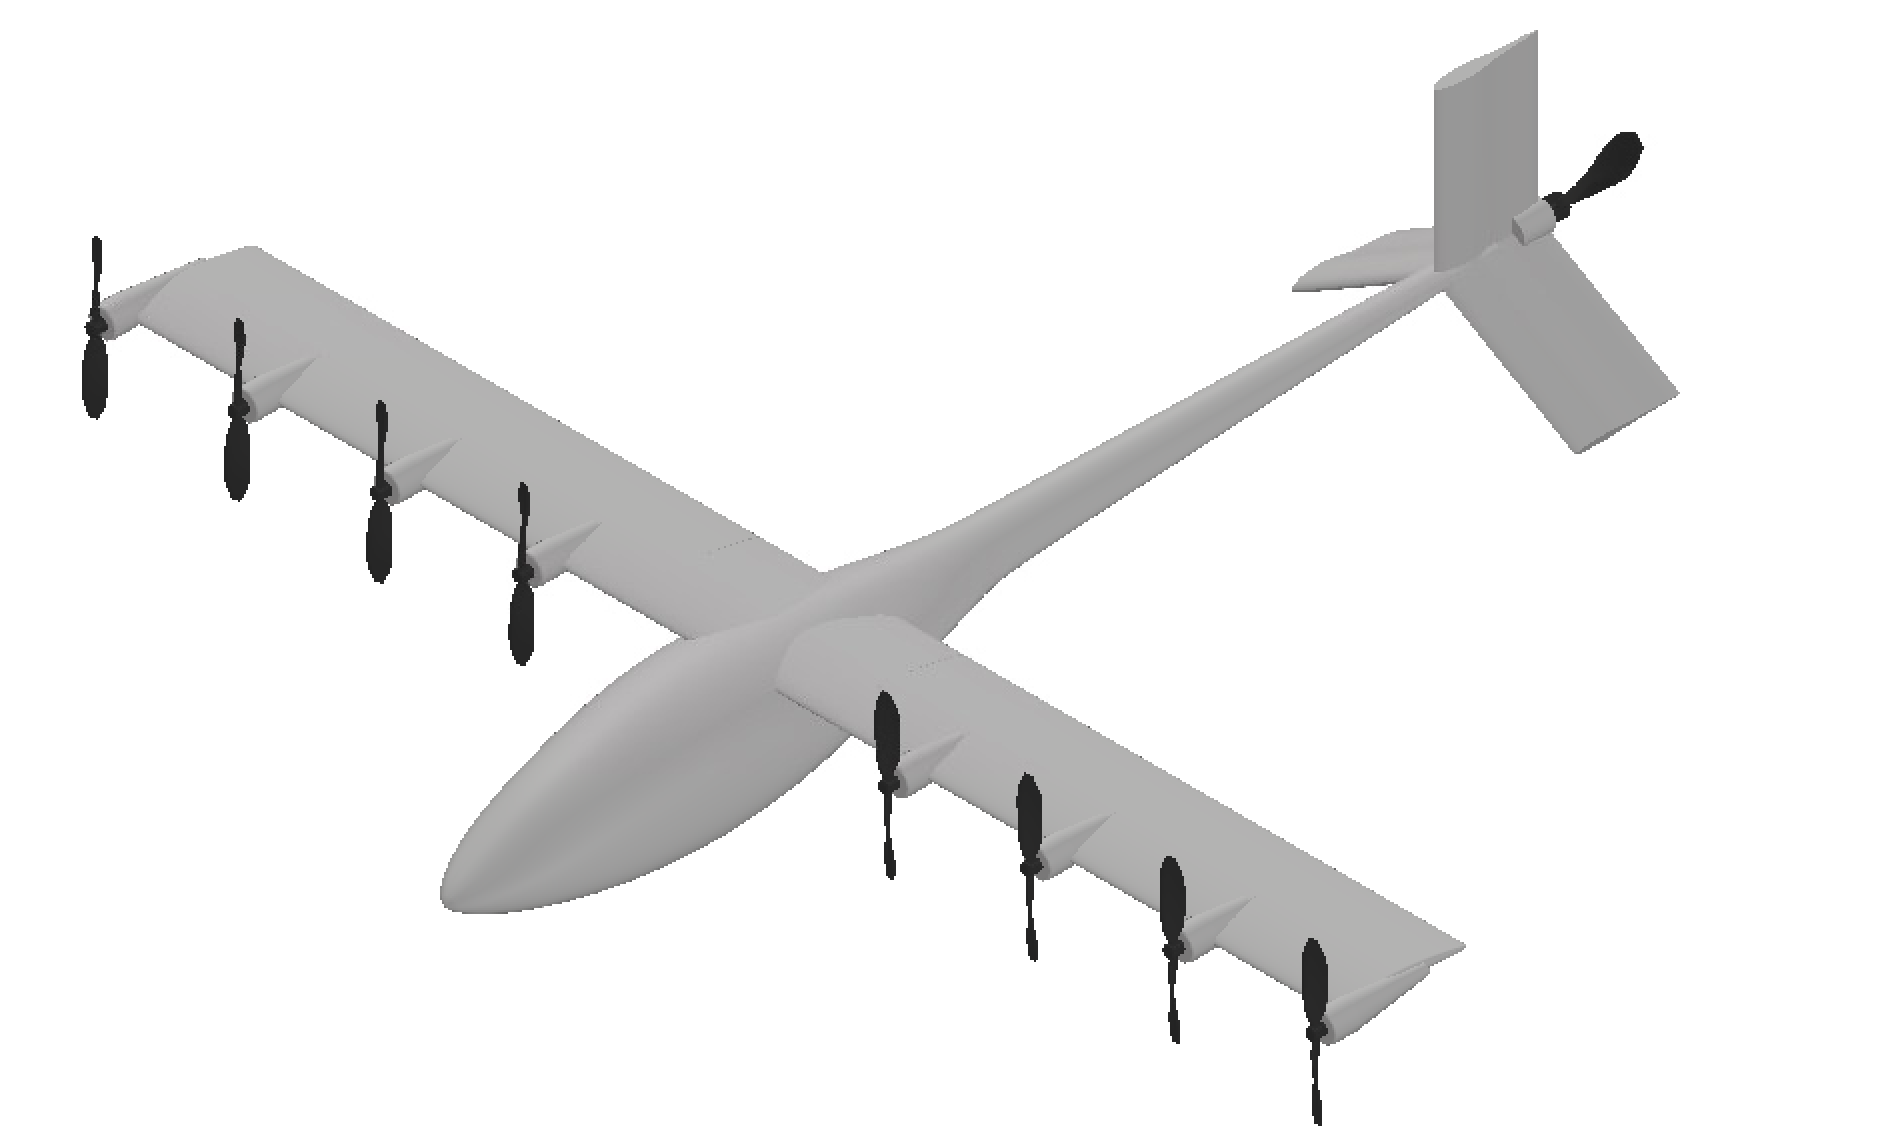
\includegraphics[width=0.95\linewidth]{Concepts/CAD/6cad.png}
  \vspace{0.125cm}
  \caption{CAD Drawing}
  \label{fig:cad3}
\end{subfigure}%
\begin{subfigure}[t]{.5\textwidth}
  \centering
  \fbox{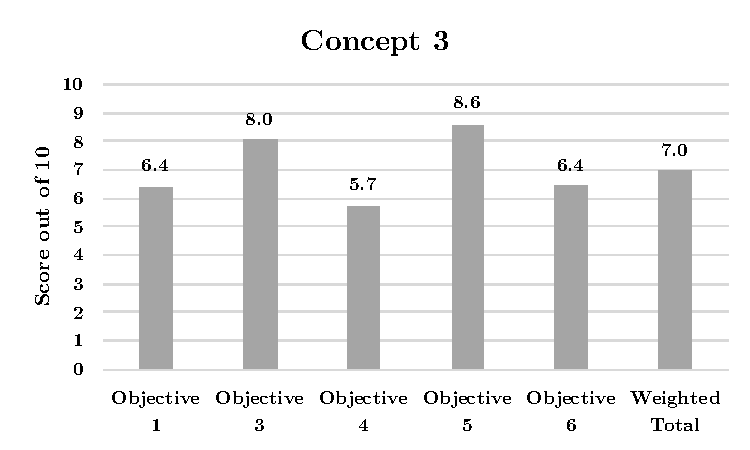
\includegraphics[width=0.95\linewidth]{Concepts/Plots/6.pdf}}
  \caption{Performance Criteria Assessment Results}
  \label{fig:radar3}
\end{subfigure}
\caption{Concept 3 - Distributed Lift Tilt Wing}
\label{fig:concept3}
\end{figure}

\paragraph{Concept 4: Distributed Propulsion and Ducted Fan Tilt-Wing Canard}
When in forward flight mode, this design uses its distributed propellers to generate lift over the main wing. During vertical flight, an integrated counter co-axial ducted fan is activated and the wings are rotated such that the distributed propellers can provide thrust and stability. Although the fan is efficient during vertical flight, it is idle during forward flight, and for it to not cause significant drag, complex covering mechanisms would need to be Incorporated. The Canard design has the potential to increase transition efficiency as it will add the positive lift being produced by the main wing, however this comes at the cost of control simplicity. This design is shown in Figure \ref{fig:concept4}



% Canard, distributed lift, tilt-wing with integrated counter co-axial rotor/fan for hover. When in forward flight, the co-axial rotor will be inactive. When in hover the counter co-axial fan will be active, opening the fuselage as depicted to produce increased thrust and improve disk area. Canard design potentially greater transition efficiency as both the canard and wing are producing positive lift, in comparison to a typical tail design which would produce negative lift; potentially hampering transition.  


\begin{figure}[H]
\centering
\begin{subfigure}[t]{.5\textwidth}
  \centering
  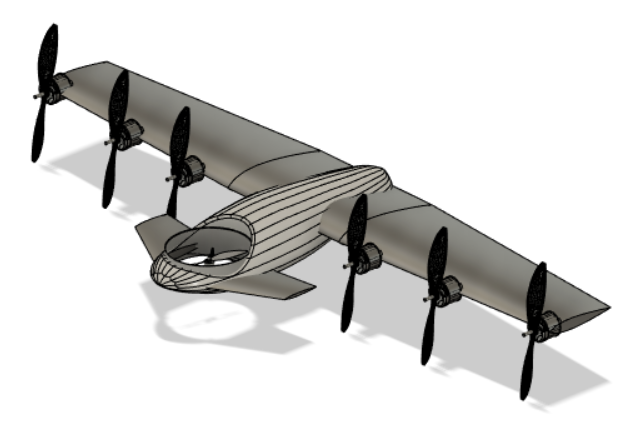
\includegraphics[width=0.9\linewidth]{Concepts/CAD/8cad.png}
  \vspace{0.125cm}
  \caption{CAD Drawing}
  \label{fig:cad4}
\end{subfigure}%
\begin{subfigure}[t]{.5\textwidth}
  \centering
  \fbox{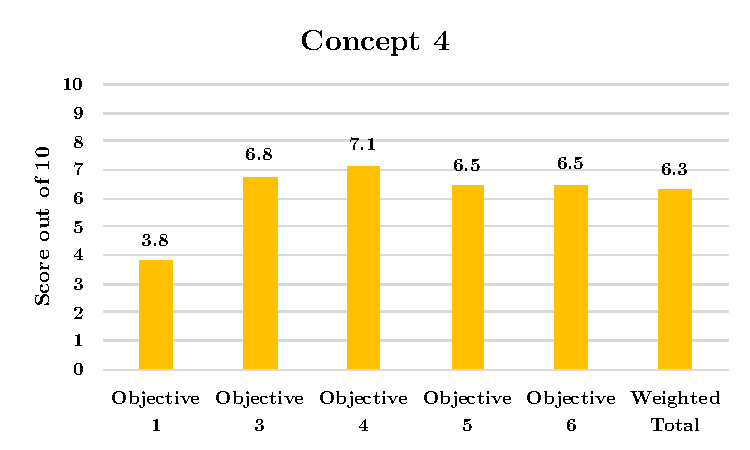
\includegraphics[width=0.95\linewidth]{Concepts/Plots/8.pdf}}
  \caption{Performance Criteria Assessment Results}
  \label{fig:radar4}
\end{subfigure}
\caption{Concept 4 - Distributed Propulsion and Ducted Fan Tilt-Wing Canard}
\label{fig:concept4}
\end{figure}

% \paragraph{Novel }
\paragraph{Concept 5: Rotor-wing Configuration}

This concept is focused around a tilt rotor-wing which allows for high aspect ratio for forward flight and high disk area for efficient hover. Like other tail sitter designs this design has limitations in scanning capabilities while in a hover configuration. It also requires a complex high precision tilt-wing/ rotor design increasing manufacturing difficulty. 


\begin{figure}[H]
\centering
\begin{subfigure}[t]{.5\textwidth}
  \centering
  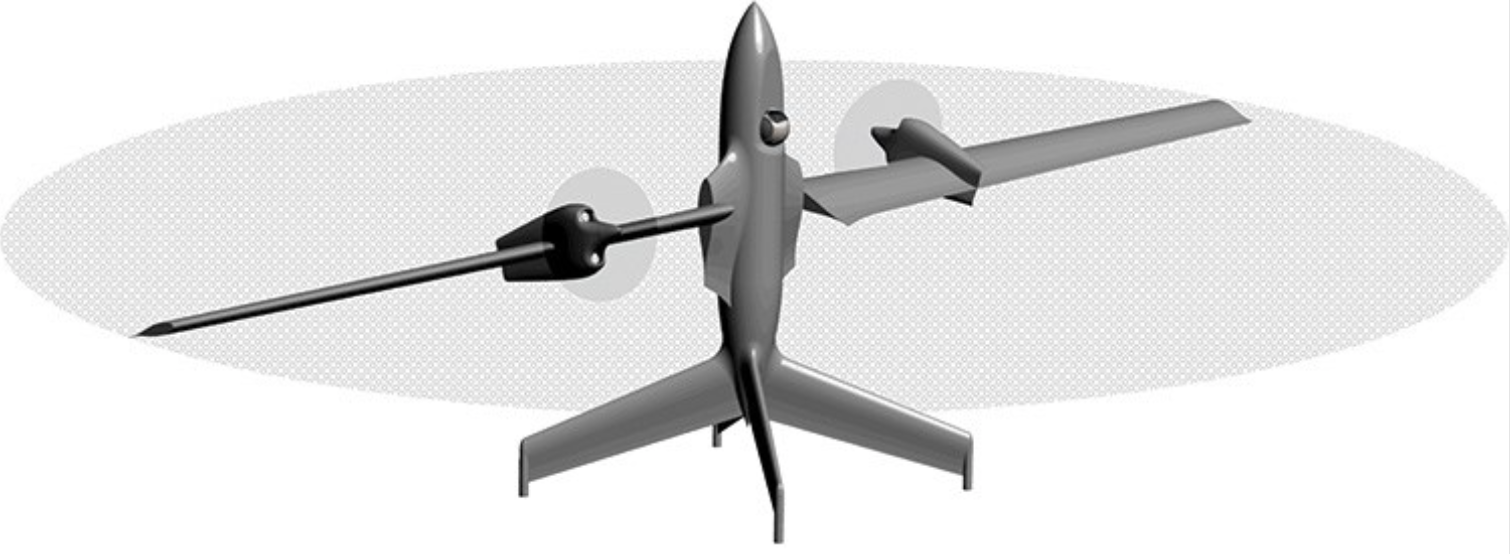
\includegraphics[width=0.9\linewidth]{Concepts/rotorwing.png}
  \vspace{0.125cm}
  \caption{CAD Model, image from }
  \label{fig:cad1}
\end{subfigure}%
\begin{subfigure}[t]{.5\textwidth}
  \centering
  \fbox{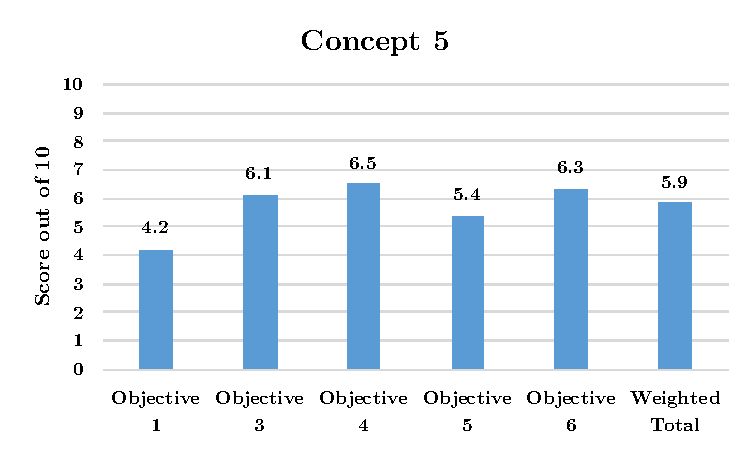
\includegraphics[width=0.95\linewidth]{Concepts/Plots/12.pdf}}
  \caption{Performance Criteria Assessment Results}
  \label{fig:radar1}
\end{subfigure}
\caption{Concept 5 - Commercially Available VTOL UAV}
\label{fig:concept2}
\end{figure}

% *A summary visual will also be provided to help compare between the concepts.
% \begin{figure}[H]
%     \centering
%     \fbox{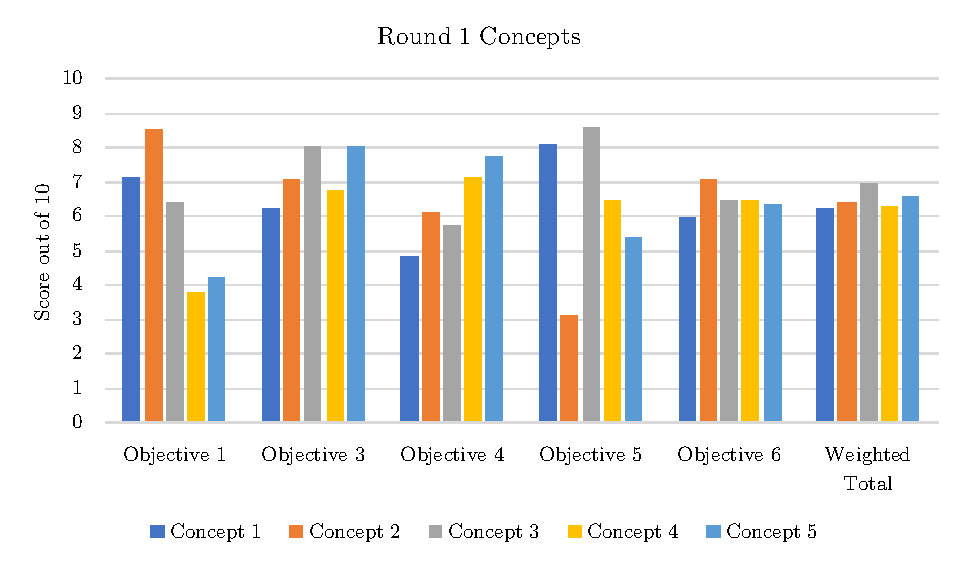
\includegraphics[width = \textwidth]{Concepts/Plots/Round1.pdf}}
%     \caption{Summary of Design for Objectives evaluation and scoring for Round 1 Concepts}
%     \label{fig:summary}
% \end{figure}

% \note{Peter}{switch objectives and concepts}

% * Further description of each concept will be displayed in the appendix. 


\subsubsection{Round 2 Concepts}
The Round 2 concepts build on the successes of Round 1, taking particular note of the performance of distributed lift designs.

% similar to round 1 concepts
% \note{Rhys}{5-[Peter],6-[Harry],7-[Jake]}

\paragraph{Concept 6: Tilt-Tip and Tilt-Tail UAV with Conventional Fuselarge}
This system comprises of a conventional fuselarge with a distributed propulsion system. The tail plane rotates along with the wing tips for stable VTOL flight. Large diameter rotor blades on the wing tips deploy on transition using centrifugal force. this allows for low disk loading for hover, increasing hover efficiency. The rotating tips and tail plane also act as a control surface to enable roll and pitch of the aircraft. This design is depicted in Figure \ref{fig:concept6}.


\begin{figure}[H]
\centering
\begin{subfigure}[t]{.5\textwidth}
  \centering
  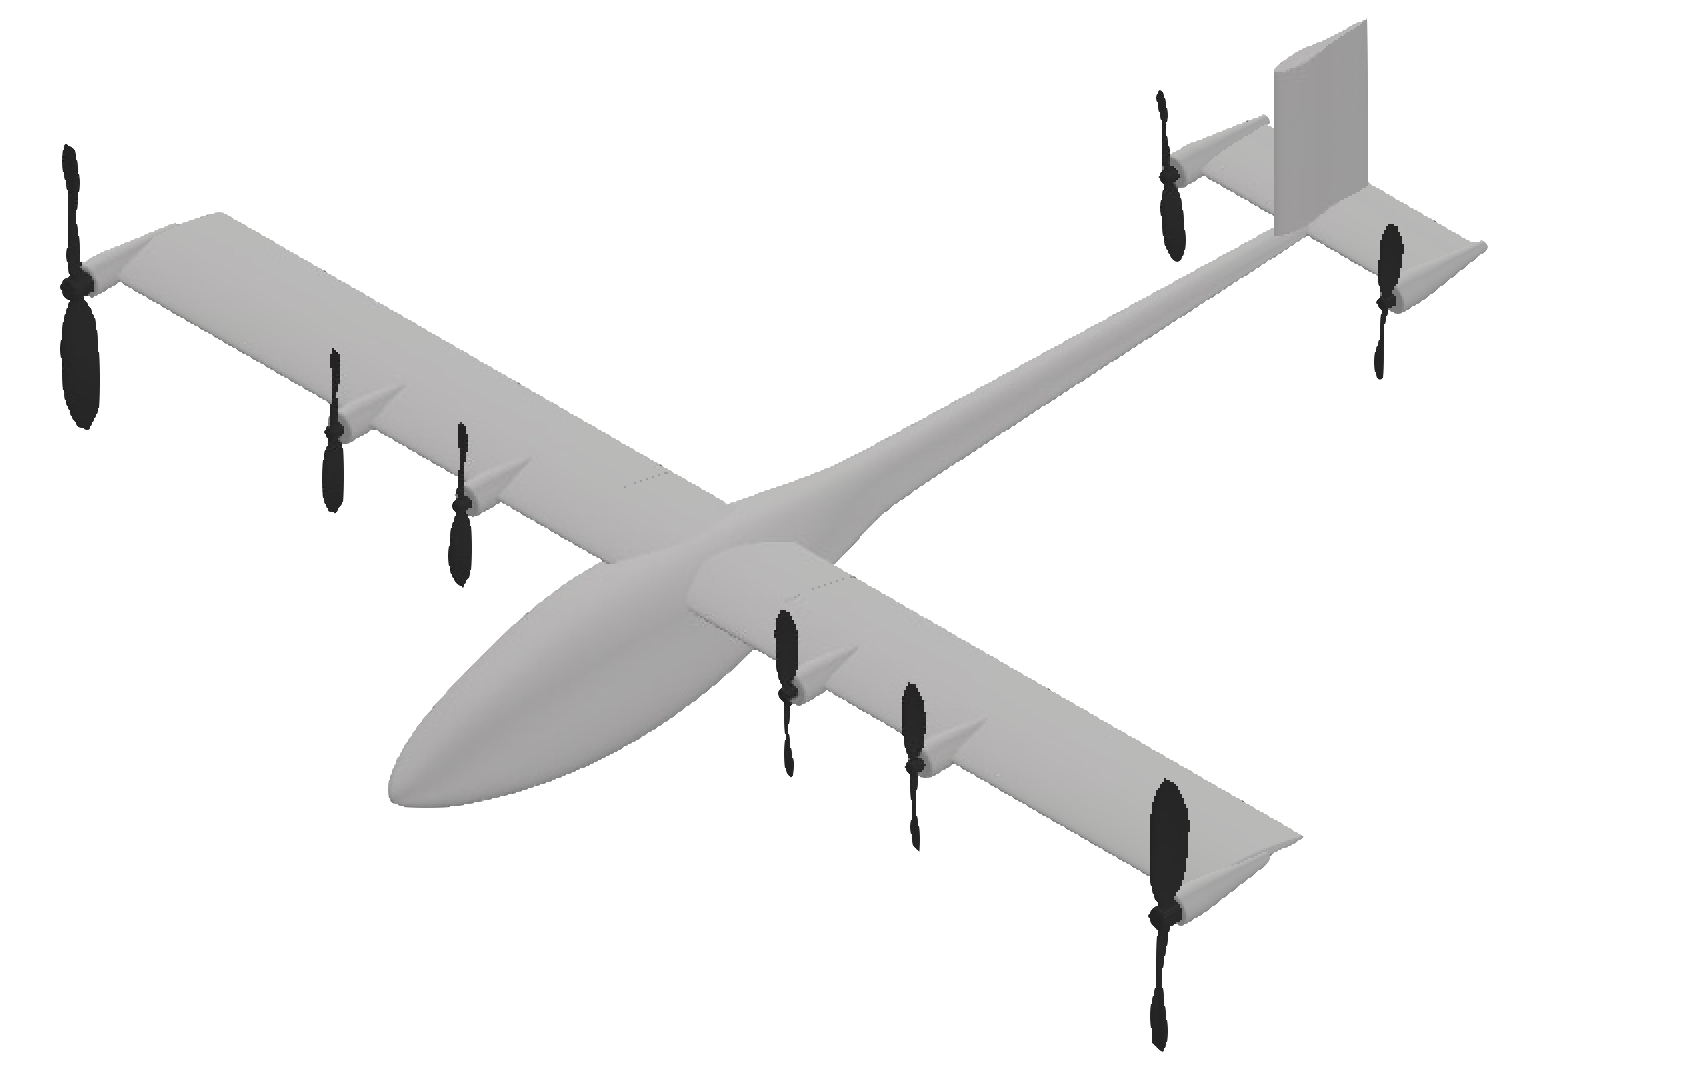
\includegraphics[width=0.95\linewidth]{Concepts/CAD/round2_1_cad.png}
  \vspace{0.125cm}
  \caption{CAD Drawing}
  \label{fig:cad6}
\end{subfigure}%
\begin{subfigure}[t]{.5\textwidth}
  \centering
  \fbox{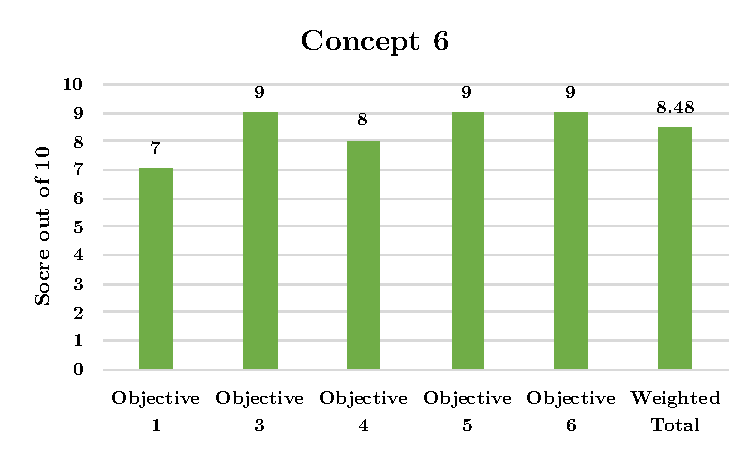
\includegraphics[width=0.95\linewidth]{Concepts/Plots/Round2_1.pdf}}
  \caption{Performance Criteria Assessment Results}
  \label{fig:radar6}
\end{subfigure}
\caption{Concept 6 - Tilt-Tip and Tail with Conventional Fuselarge}
\label{fig:concept6}
\end{figure}

\paragraph{Concept 7: Tilt-Rotor with Co-Axial Ducted Fan}
This concept incorporates a tilt rotor design with integrated counter co-axial ducted fan. The tilt rotors act as pushers and can tilt independently to aid with control. A covering opens and closes over the duct to streamline the design depending on the current flightmode. Further investigation is required to realise the optimal location of the co-axial rotor. This design is shown in Figure \ref{fig:concept7}.

\begin{figure}[H]
\centering
\begin{subfigure}[t]{.5\textwidth}
  \centering
  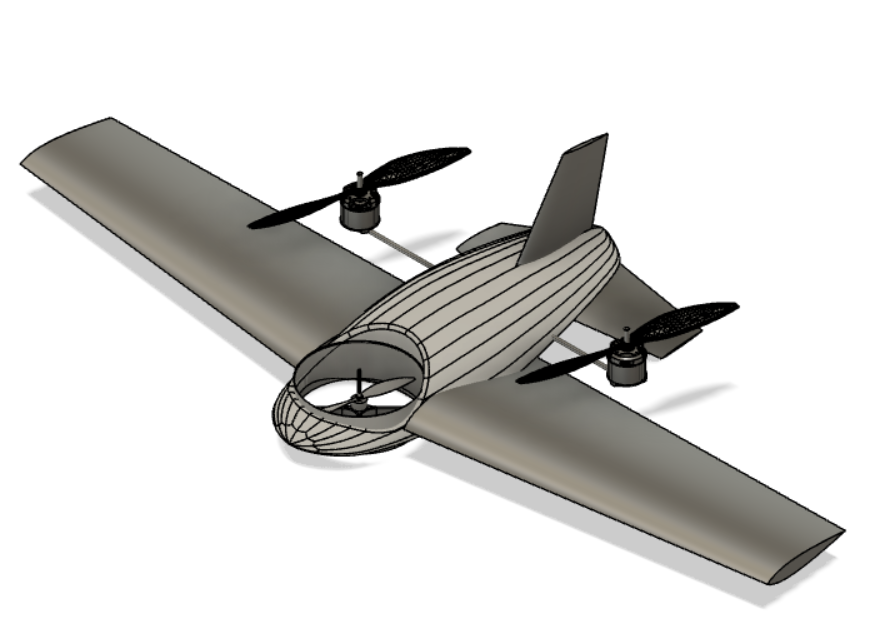
\includegraphics[width=0.95\linewidth]{Concepts/CAD/Round2_2_cad.png}
  \vspace{0.125cm}
  \caption{CAD Drawing}
  \label{fig:cad7}
\end{subfigure}%
\begin{subfigure}[t]{.5\textwidth}
  \centering
  \fbox{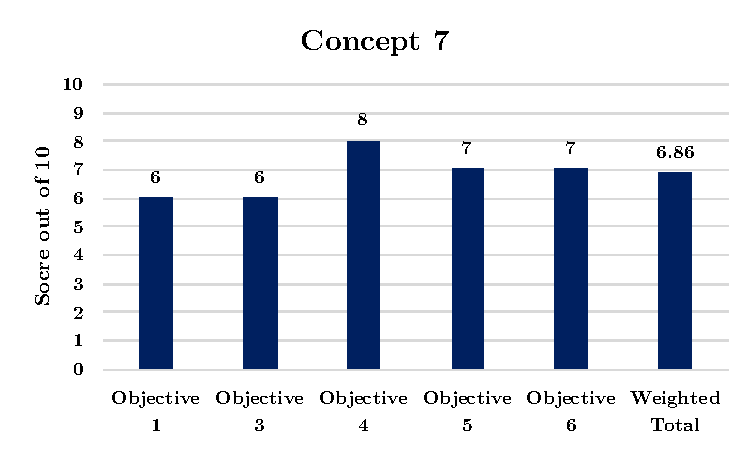
\includegraphics[width=0.95\linewidth]{Concepts/Plots/Round2_2.pdf}}
  \caption{Performance Criteria Assessment Results}
  \label{fig:radar7}
\end{subfigure}
\caption{Concept 7 - Tilt-Rotor with Co-Axial Ducted Fan}
\label{fig:concept7}
\end{figure}


\paragraph{Concept 8: Tilt-Wing Canard Distributed Lift Design}
This design achieves distributed lift with smaller, more efficient motors by overlapping the propeller disk areas. This increases efficiency of lift generation during forward flight, and also increases disk area and hence efficiency during vertical flight. The tilt-wing mechanism is housed within the fuselarge to minimise drag. Figure \ref{fig:concept8} depicts this design.


% Canard design, tilt-wing/canard, distributed lift aircraft. Tilting mechanism housed at each wing's joint to the main fuselage. Distributed lift system acts as thrust for both VTOL, hover and forward flight, using smaller but more efficient motors and by overlapping disk areas of props will increase efficiency of lift generation, as well as increase disk area and improve hover efficiency. Can possibly include a system to deactive certain motors on the wing to save power if required. 



\begin{figure}[H]
\centering
\begin{subfigure}[t]{.5\textwidth}
  \centering
  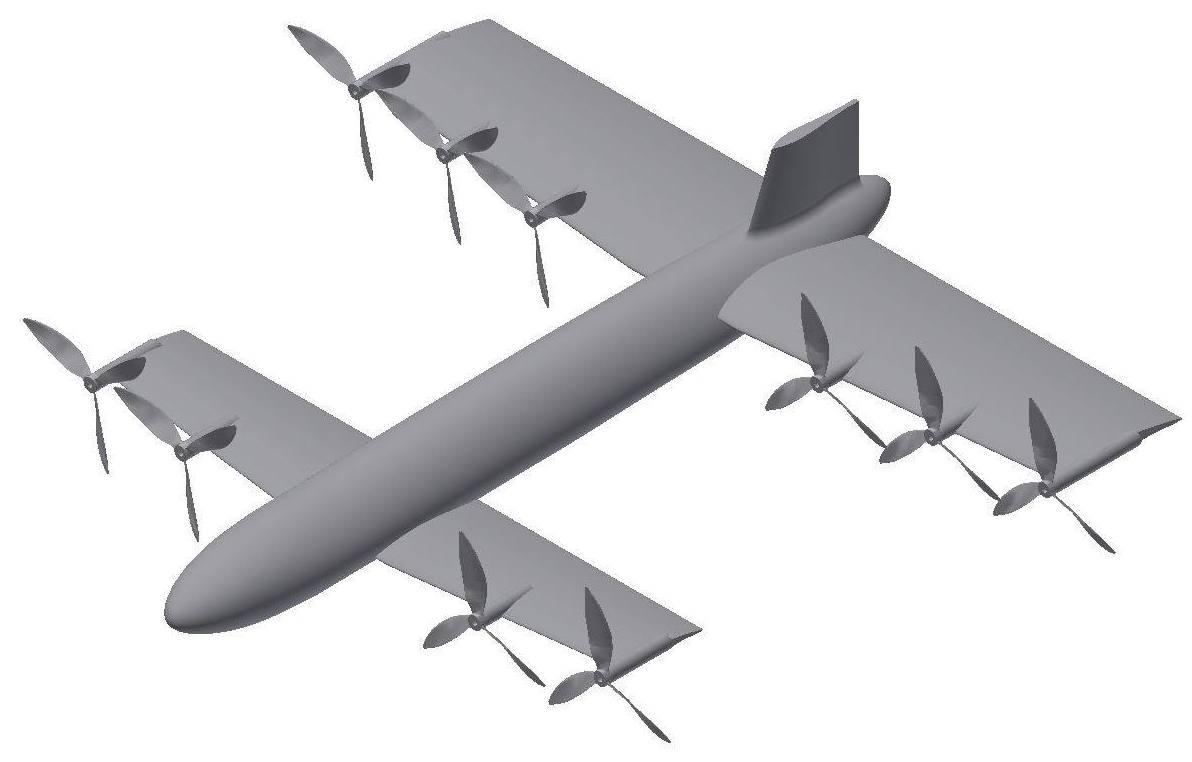
\includegraphics[width=0.95\linewidth]{Concepts/CAD/Round2_3_cad.jpg}
  \vspace{0.125cm}
  \caption{CAD Drawing}
  \label{fig:cad8}
\end{subfigure}%
\begin{subfigure}[t]{.5\textwidth}
  \centering
  \fbox{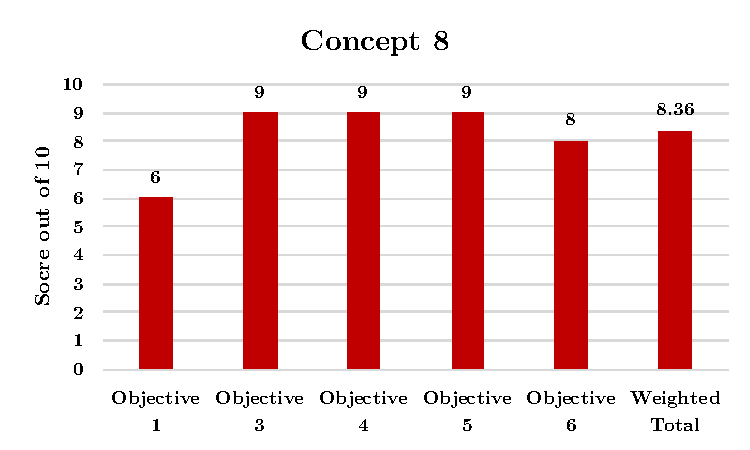
\includegraphics[width=0.95\linewidth]{Concepts/Plots/Round2_3.pdf}}
  \caption{Performance Criteria Assessment Results}
  \label{fig:radar8}
\end{subfigure}
\caption{Concept 8 - Tilt-Wing Canard Distributed Lift Design}
\label{fig:concept8}
\end{figure}

% \begin{figure}[H]
%     \centering
%     \fbox{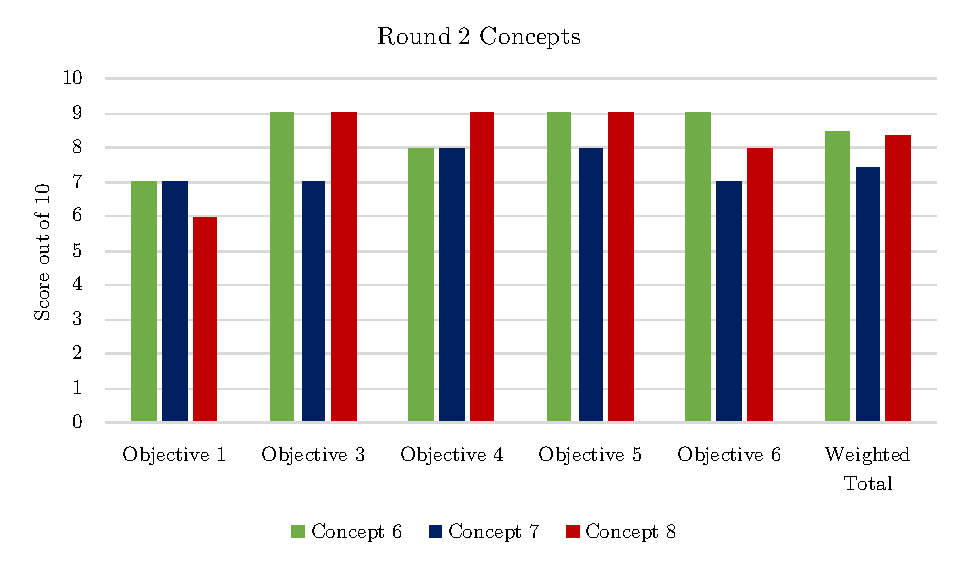
\includegraphics[width = \textwidth]{Concepts/Plots/Round2.pdf}}
%     \caption{Summary of Design for Objectives evaluation and scoring for Round 1 Concepts}
%     \label{fig:summary}
% \end{figure}


\subsubsection{Round 3 Concepts}
Based on the efficiency benefits of ducted fans and distributed lift configurations, concepts featuring these technologies were further explored.

\paragraph{Concept 9: Canard with Ducted Fans}
This design features a counter co-axial fan incorporated into the front section of the fuselarge and ducted fans mounted in the wings. This has the advantage of reducing the frontal area causing drag of the ducted fans. The main wing has the ability to tilt, allowing all ducts to be used during vertical flight. This design is shown in Figure \ref{fig:concept9}

\begin{figure}[H]
\centering
\begin{subfigure}[t]{.5\textwidth}
  \centering
  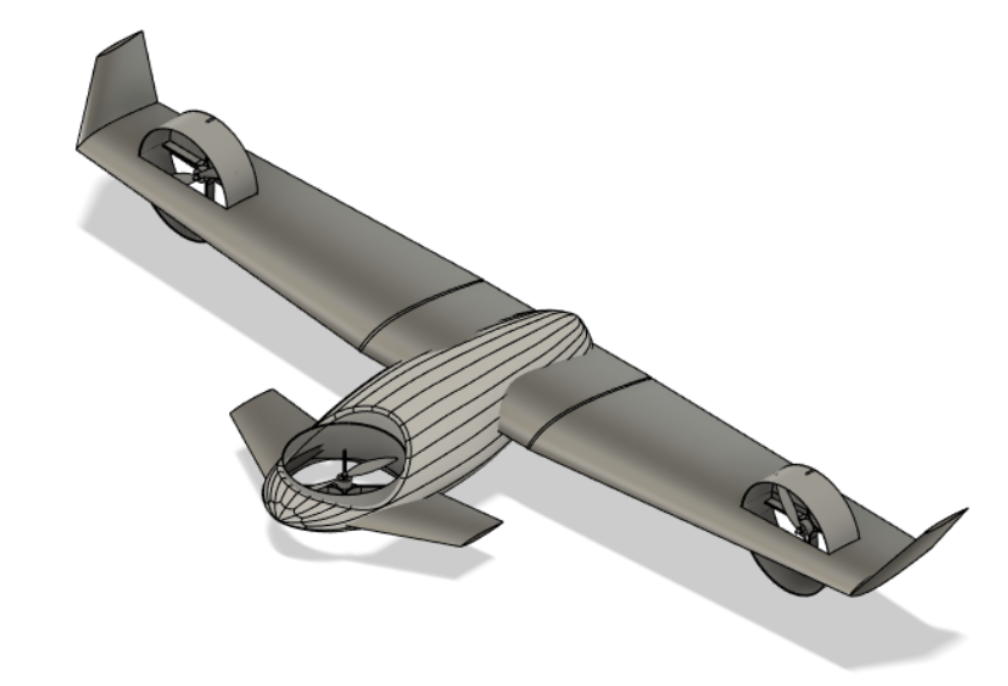
\includegraphics[width=0.95\linewidth]{Concepts/CAD/Round3_1.png}
  \vspace{0.125cm}
  \caption{CAD Drawing}
  \label{fig:cad9}
\end{subfigure}%
\begin{subfigure}[t]{.5\textwidth}
  \centering
  \fbox{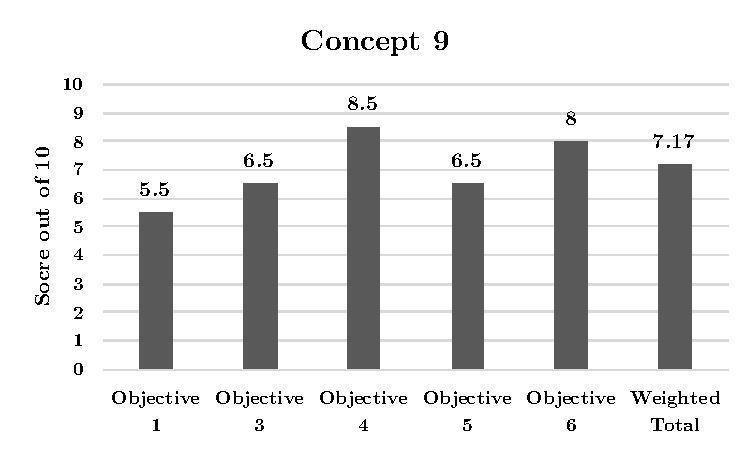
\includegraphics[width=0.95\linewidth]{Concepts/Plots/9.pdf}}
  \caption{Performance Criteria Assessment Results}
  \label{fig:radar9}
\end{subfigure}
\caption{Concept 9 - Canard with Ducted Fans}
\label{fig:concept9}
\end{figure}



\begin{figure}[H]
\centering
\begin{subfigure}[t]{.5\textwidth}
  \centering
  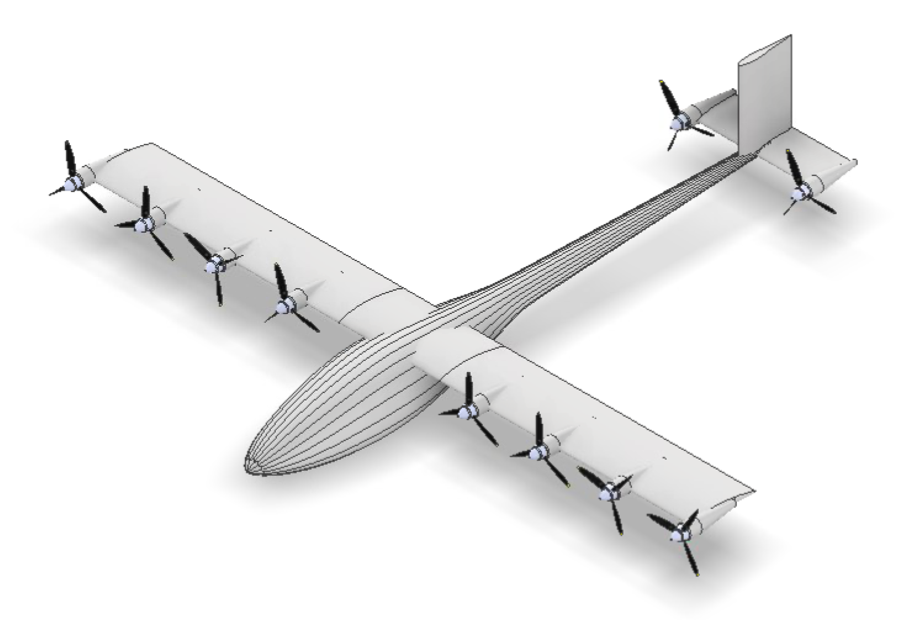
\includegraphics[width=0.95\linewidth]{Concepts/CAD/Round3_2.png}
  \vspace{0.125cm}
  \caption{CAD Drawing}
  \label{fig:cad1}
\end{subfigure}%
\begin{subfigure}[t]{.5\textwidth}
  \centering
  \fbox{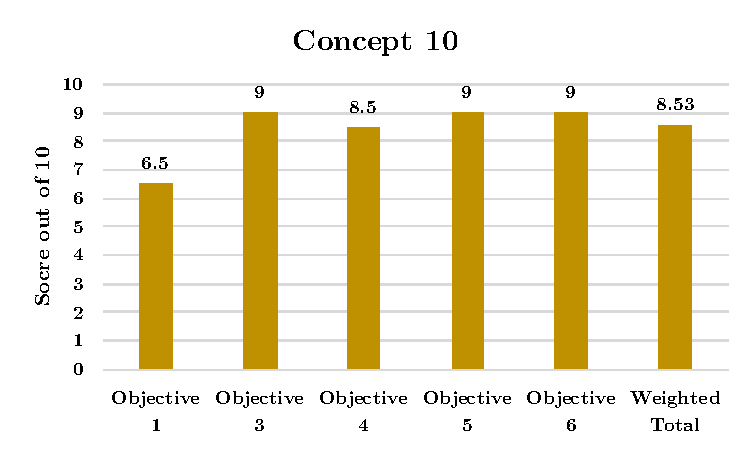
\includegraphics[width=0.95\linewidth]{Concepts/Plots/10.pdf}}
  \caption{Performance Criteria Assessment Results}
  \label{fig:radar1}
\end{subfigure}
\caption{Concept 5 - Commercially Available VTOL UAV}
\label{fig:concept2}
\end{figure}



\subsection{Concept Generation Approach Performance}

Plotting the results for all concepts in chronological order as seen in Figure \ref{fig:concept_summary} highlights a positive trend in performance. This suggests that the concept generation process was successful and achieved its aim of finding an design optimised for the project objectives. 

\begin{figure}[H]
    \centering
    \fbox{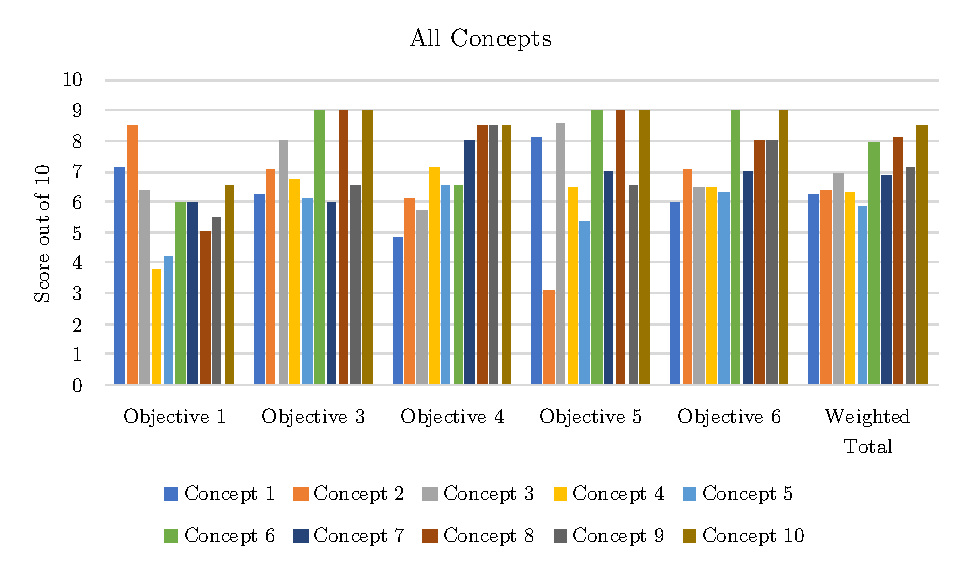
\includegraphics[width = \textwidth]{Concepts/Plots/All.pdf}}
    \caption{Improvement achieved during concept generation rounds}
    \label{fig:concept_summary}
\end{figure}

Figure \ref{fig:improvement} further demonstrates the level of improvement after each round. The scores for Objective 1, Design and Manufacture and Airframe, are seen to stay fairly consistent throughout the rounds. As this is not a key area of innovation for the project, that is an acceptable outcome. In contrast, Objectives 3 and 4 (pertaining to forward and vertical fight modes) see an improvement of 13\% and 40\% respectively between Round 1 and 3 on average.

\begin{figure}[H]
    \centering
    \fbox{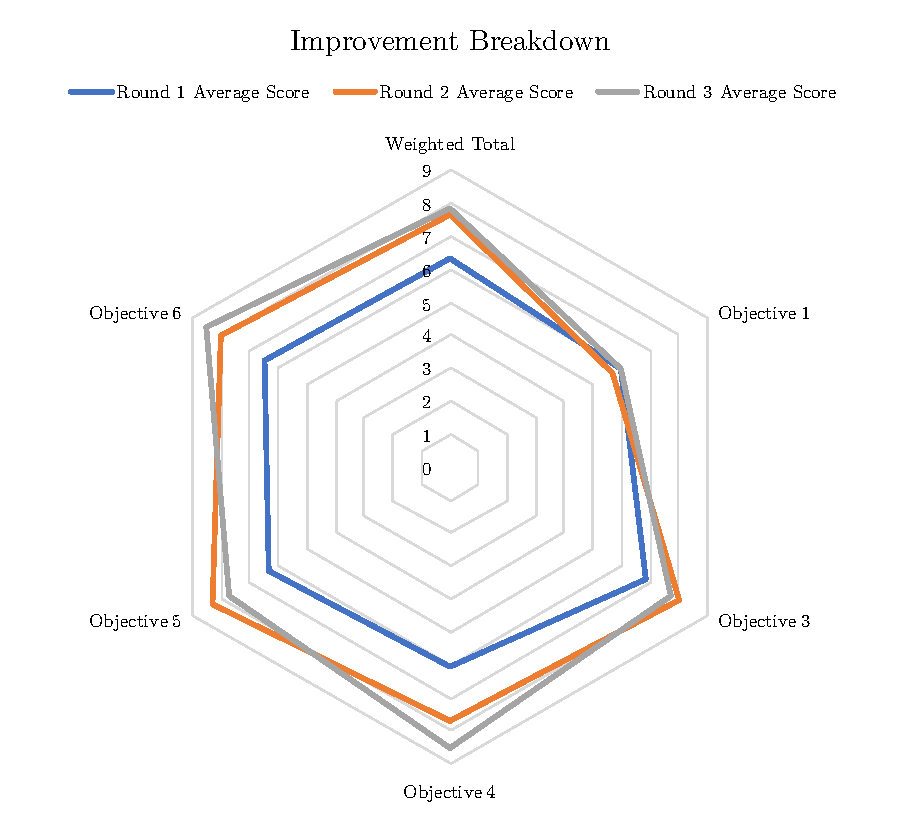
\includegraphics[width = 0.8\textwidth]{Concepts/Plots/Improvement.pdf}}
    \caption{Improvement achieved during concept generation rounds}
    \label{fig:improvement}
\end{figure}

\subsection{Final Concept}
% \note{Rhys}{Final concept that we present to Craig - [Harry]}

The concept generation process concluded that the most suitable airframe design was that of a canard. Despite inherent manufacturing and design difficulties indicated when assessing against Objective 1 compared to the conventional, this configuration offered the best balanced performance between forward flight, hover flight and flight mode transitioning. In addition to this, the canard configuration is supported by literature to be more aerodynamically efficient, as the result of all lifting surfaces being used to produced positive lift (\citeauthor{marques2013flight, \citeyear{marques2013flight}}).  

%The final design is based upon a canard configuration which utilises a tilt wing mechanism and modular wings to allow for continuing analysis in optimum propulsion system. 

%Based on the results from the concept generation and analysis, the team are looking to prototype a tilt-wing canard design that leverages the benefits of distributed propulsion using propellers mounted the all four aerofoils. This will likely be similar to Concept 8.\\
